%!TEX root = ../scivis_lbaakman_bvanloon.tex
\chapter{Gradients} % (fold)
\label{cha:gradients}
In the previous chapters we covered the various datasets in the simulation; the fluid density, fluid velocity, and the force field. In this chapter we discuss how two new datasets are created using the existing data: the fluid density gradient and the fluid velocity gradient. Gradients are multi-variable generalization of derivatives and are a function of change on the associated dataset. Gradients are vector field with vectors composed of the direction of greatest change and amount of change in that direction. Since the gradients are not directly represented, they have to inferred from the existing data.

\section{Calculating Gradients} % (fold)
\label{sec:calculating_gradients}
Calculation of the fluid density gradient is done using the cells discussed in \cref{cha:glyphs}. The gradient of a point on the grid is calculated by looking at the difference between the values of vertices of the cell containing that point and linear interpolating this difference based on the position of the point in the cell. Similar to the interpolation of the vector data, the gradient vector can be interpolated by interpolating the $x$ and $y$ components independently, thus: 
\begin{align*}
\Delta \begin{bmatrix}x\\y \end{bmatrix} = \begin{bmatrix}\Delta x\\\Delta y \end{bmatrix} .
\end{align*}

Given the scalar values at the four cell vertices:
\begin{itemize}
	\item $UL$ for the upper left vertex
	\item $UR$ for the upper right vertex
	\item $BL$ for the bottom left vertex
	\item $BR$ for the bottom right vertex
\end{itemize}
the gradient on point $p$ is calculated as given in \cref{eq:gradient}

\begin{align}\label{eq:gradient}
	\Delta x = (1 - p_y) * \frac{BR - BL}{C_w} +
      p_y * \frac{UR - UL}{C_w}\\
	\Delta y = (1 - p_x) * \frac{UL - BL}{C_h} +
      p_y * \frac{UR - BR}{C_w}\\
\end{align}
This method can be used for both the gradient of the fluid density as well as the gradient of the fluid velocity magnitude.

\section{Visualization of Gradients} % (fold)
\label{sec:visualization_of_gradients}
Since the gradients are vector data, containing both direction and magnitude, they are best visualized using the Glyphs presented in \cref{cha:glyphs}. In \cref{fig:gradients} a visualization is given of both the fluid density gradient as the fluid velocity gradient using the cold colormap visualization of the fluid density as background. Looking at the glyphs of the fluid density gradient in \cref{fig:gradients:density} we see that the glyphs point towards the two areas which have the highest gradient according to the colormap. The fluid velocity gradient displayed in \cref{fig:gradients:velocity} appears to be pointing in the opposite direction of the fluid density gradient. Thus fluid moves away from locations which have a relative high density. This effect is even better noticeable when we zoom in on an area with high fluid density.
\begin{figure}[tbh]
	\centering
	\begin{subfigure}{0.45\textwidth}
		\centering
		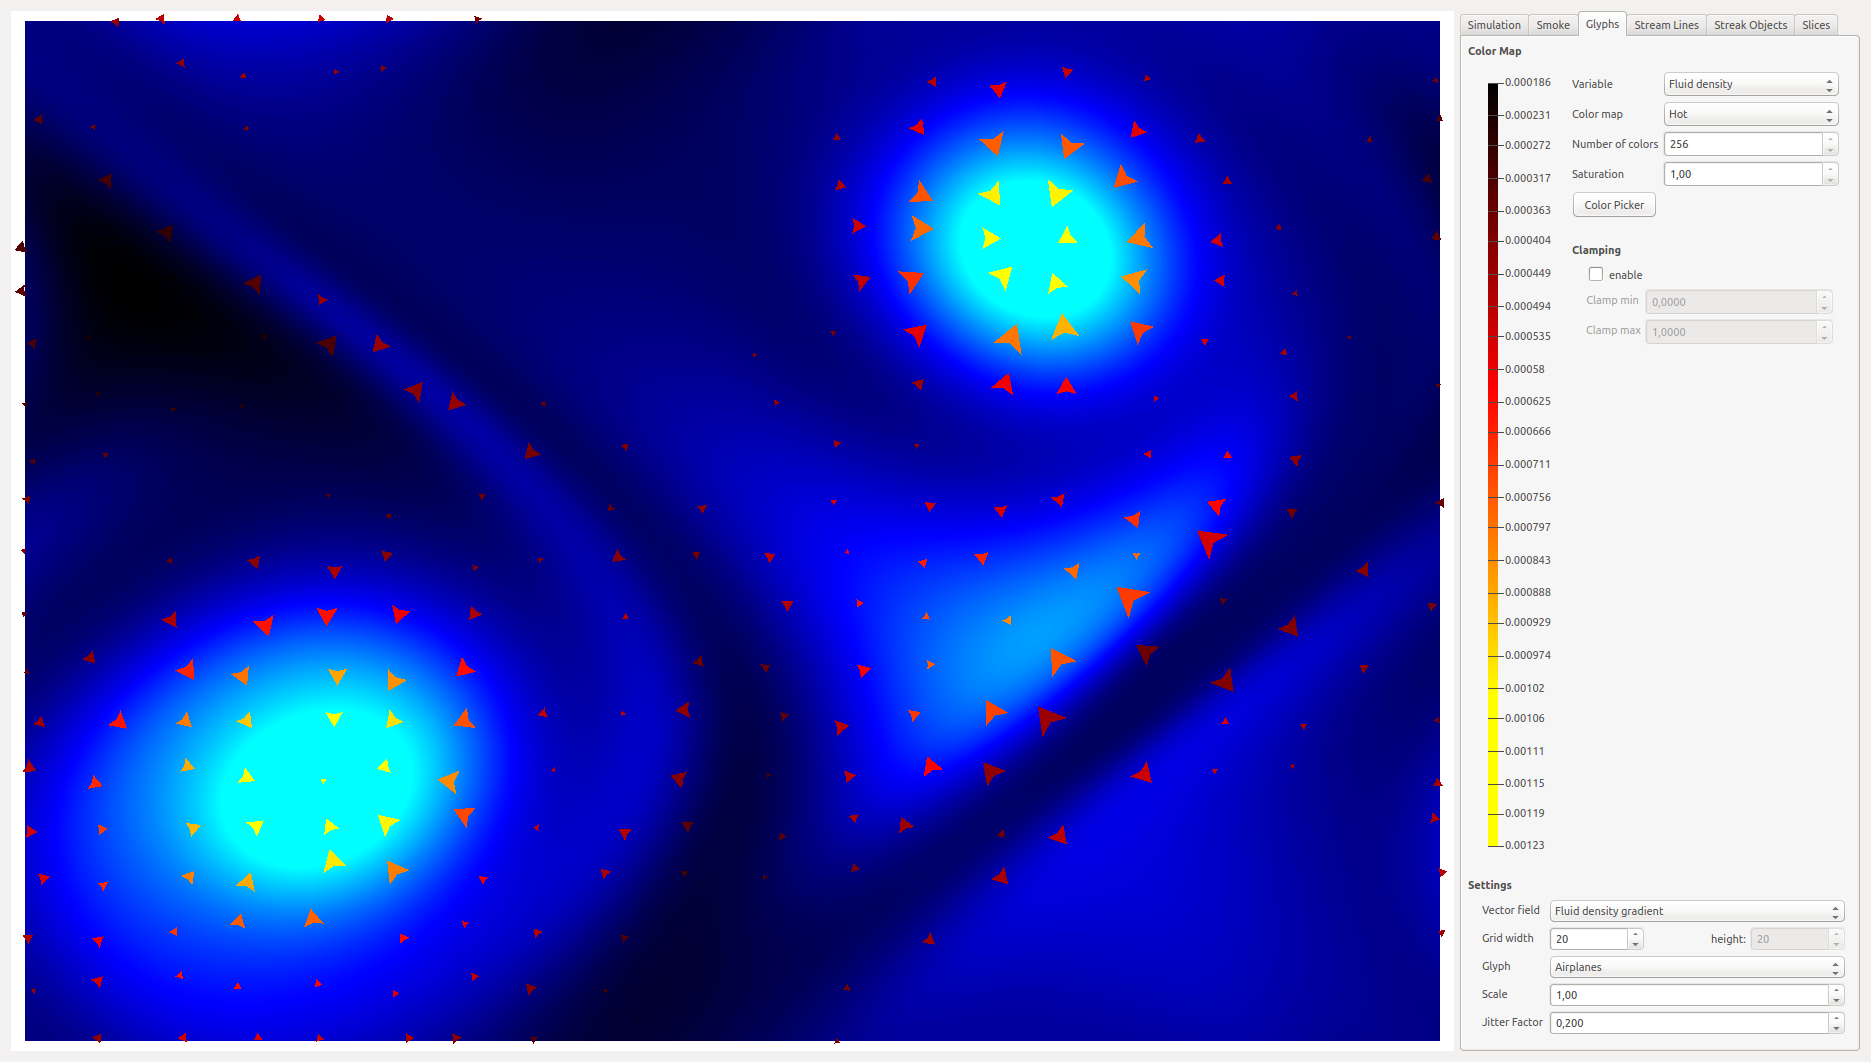
\includegraphics[width=0.9\textwidth, trim={35px 30px 430px 30px}, clip]{img/gradient/fluid_density_gradient}
		\caption{The fluid density (cold colormap) overlaid with airplane glyphs showing the fluid density gradient using the heat colormap.}
		\label{fig:gradients:density}
	\end{subfigure}
	\hspace{30px}
	\begin{subfigure}{0.45\textwidth}	
		\centering
		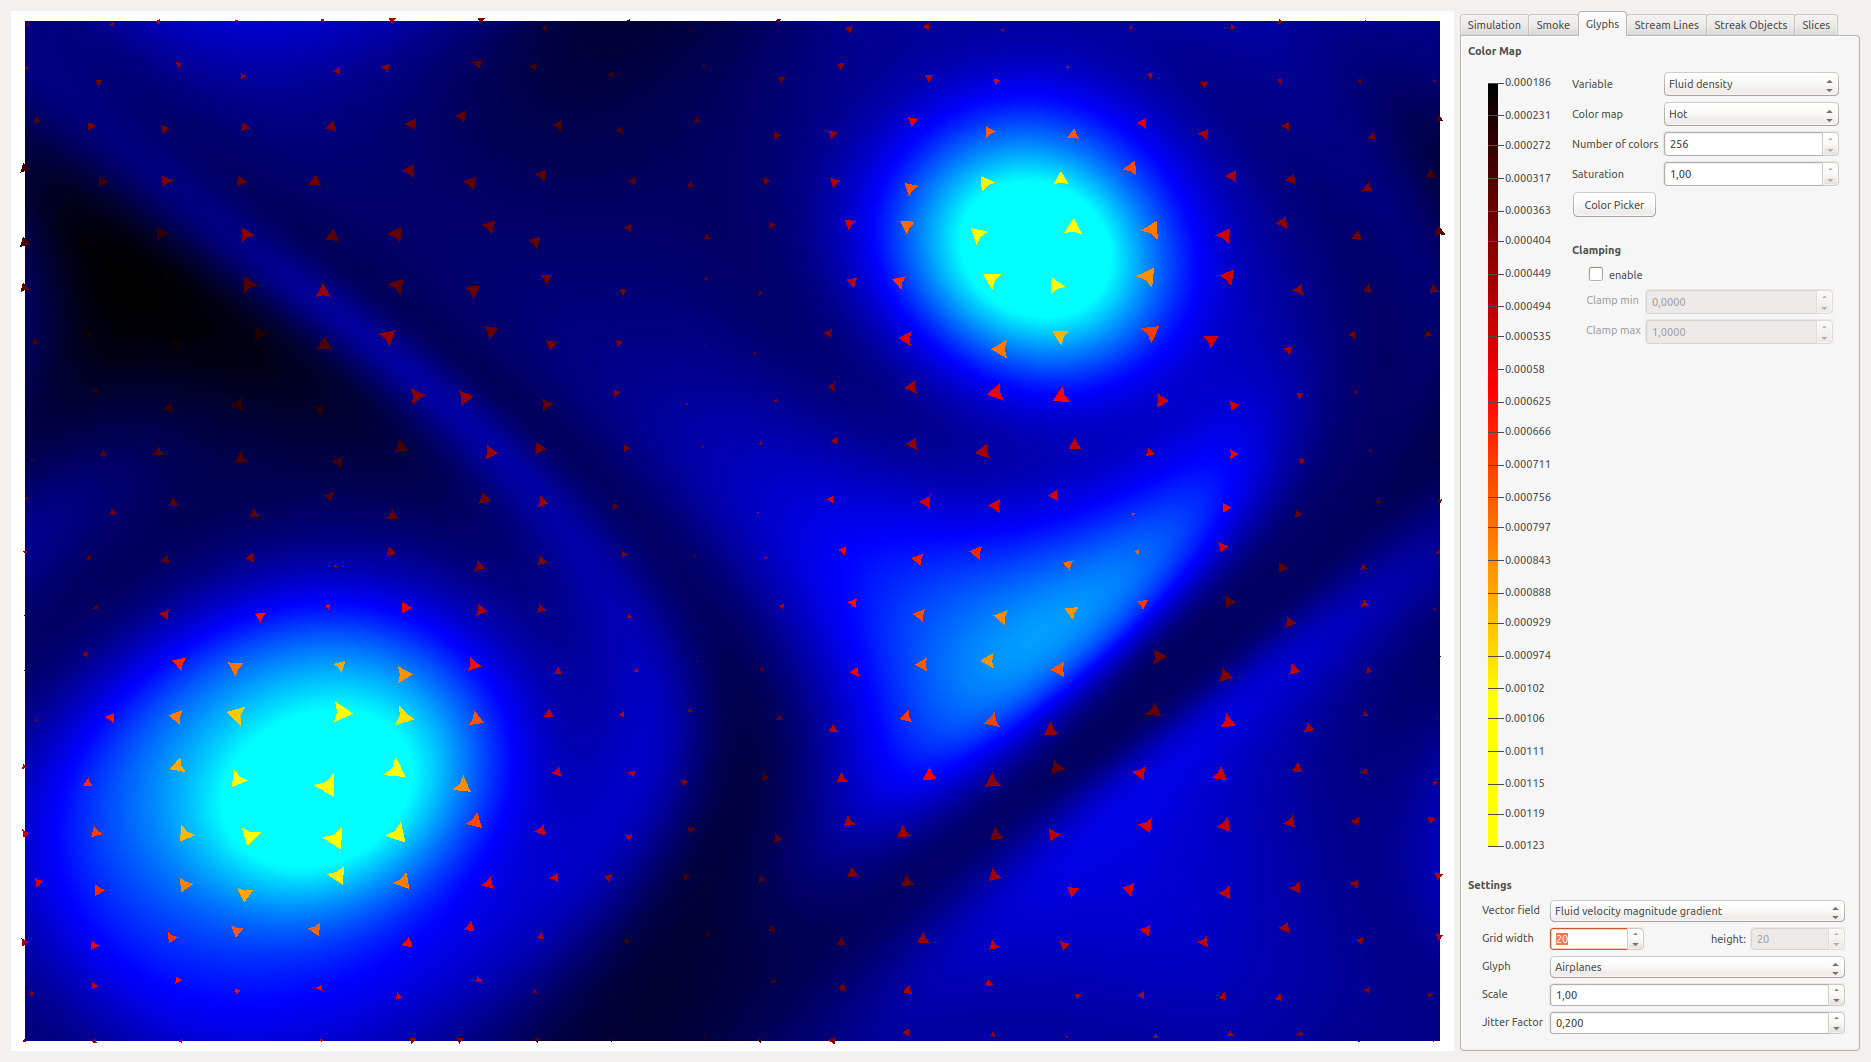
\includegraphics[width=0.9\textwidth, trim={35px 30px 430px 30px}, clip]{img/gradient/fluid_velocity_gradient}
		\caption{The fluid density (cold colormap) overlaid with airplane glyphs showing the fluid velocity gradient using the heat colormap.}
		\label{fig:gradients:velocity}
	\end{subfigure}
	\caption{The difference between the fluid velocity gradient and fluid density gradient. Both visualization have the fluid density as background using the cold colormap and use the heat colormap for the glyphs. Both visualization use airplane glyphs on a 20 by 20 grid using a jitter-factor of 0.2.}
	\label{fig:gradients}
\end{figure}

\begin{figure}[tbh]
	\centering
	\begin{subfigure}{0.45\textwidth}
		\centering
		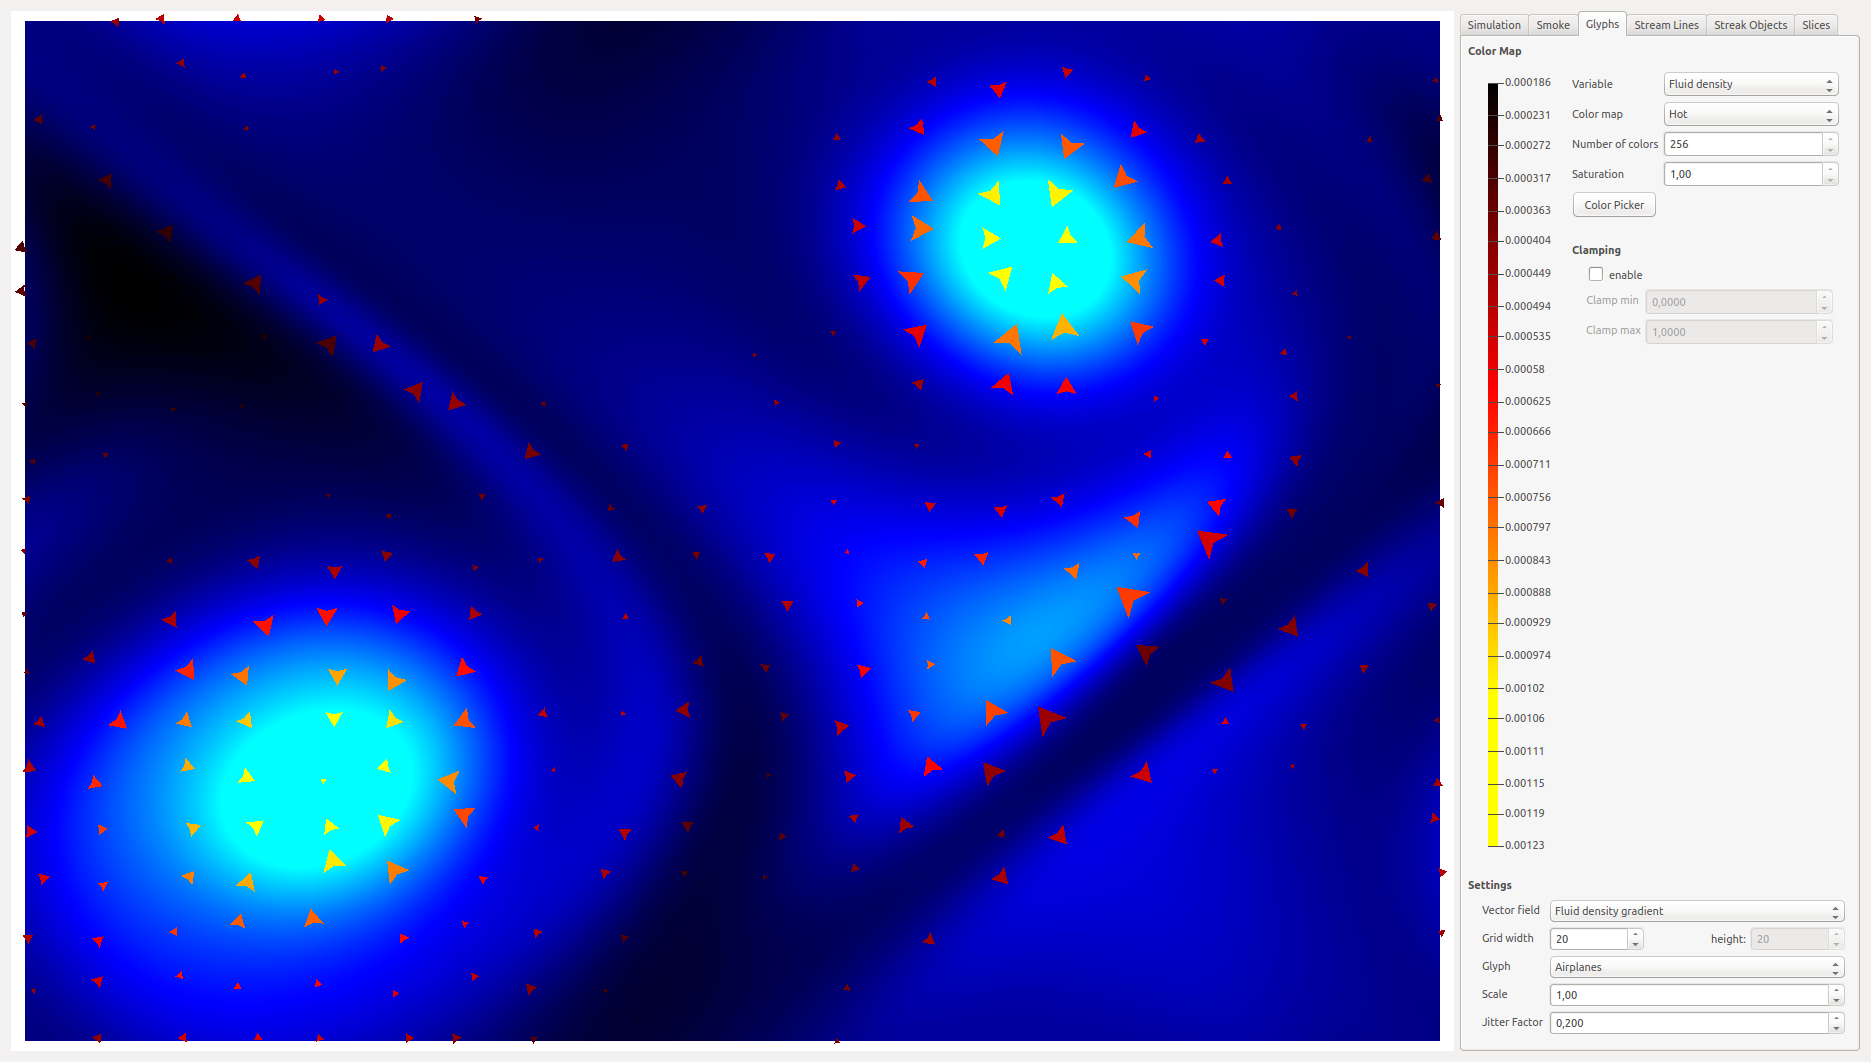
\includegraphics[width=0.9\textwidth, trim={35px 30px 1076px 500px}, clip]{img/gradient/fluid_density_gradient}
		\caption{Fluid density gradient shown in \cref{fig:gradients:density}, zoomed in on an area with max density.}
		\label{fig:gradients:zoom:density}
	\end{subfigure}
	\hspace{30px}
	\begin{subfigure}{0.45\textwidth}	
		\centering
		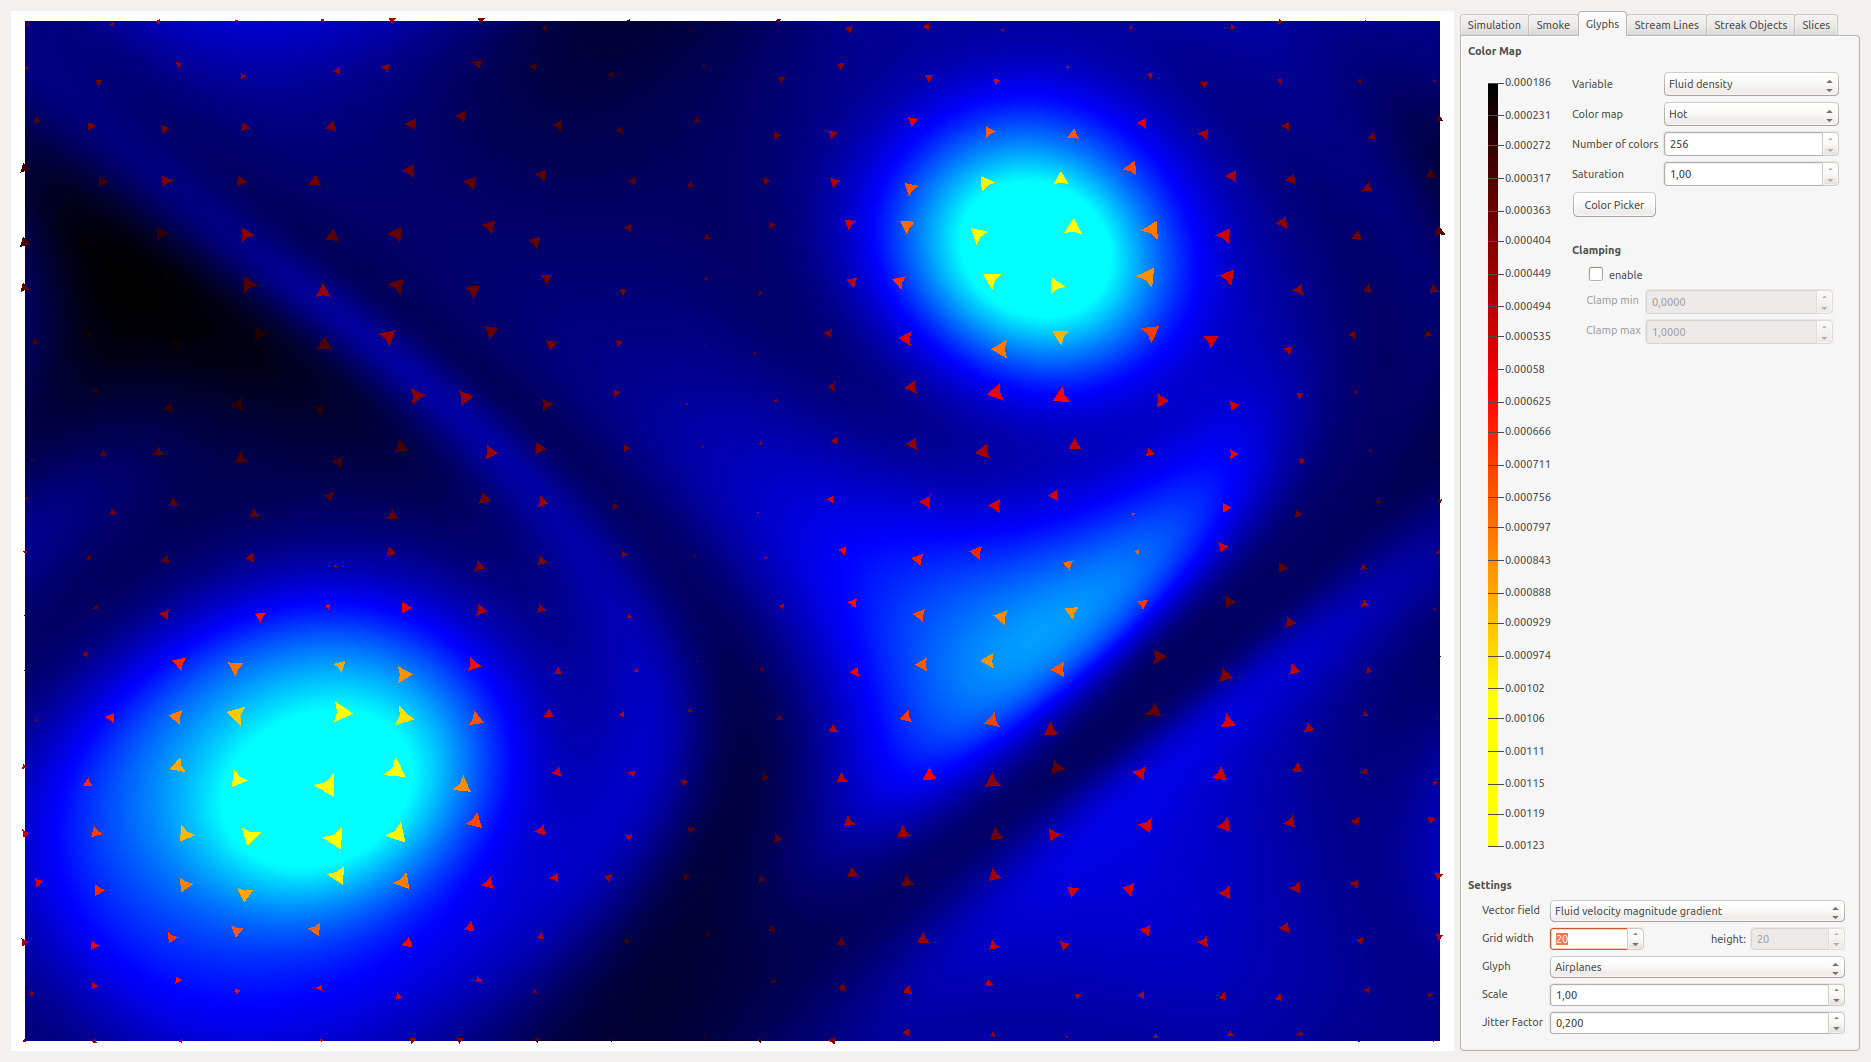
\includegraphics[width=0.9\textwidth, trim={35px 30px 1076px 500px}, clip]{img/gradient/fluid_velocity_gradient}
		\caption{Fluid density gradient shown in \cref{fig:gradients:velocity}, zoomed in on an area with max density.}
		\label{fig:gradients:zoom:velocity}
	\end{subfigure}
	\caption{A zoomed in version of \cref{fig:gradients} showing one of the areas with the highest density.}
	\label{fig:gradients:zoom}
\end{figure}